
\chapter{Basic Reinforcement Learning Example Using Logistic Regression }
\label{chapter:logistic-regression}

Logistic Regression is one of the methods that can be used as an activation function. Others include Rectified Linear Units (ReLU) and the Perceptron. The conceptual target of using this activation function is to achieve the all mighty goal of linear separability. The data can be transformed through the activation function to find a hyperplane that can separate the data nicely. 

\begin{figure}
	\label{figure:logistic-function}
	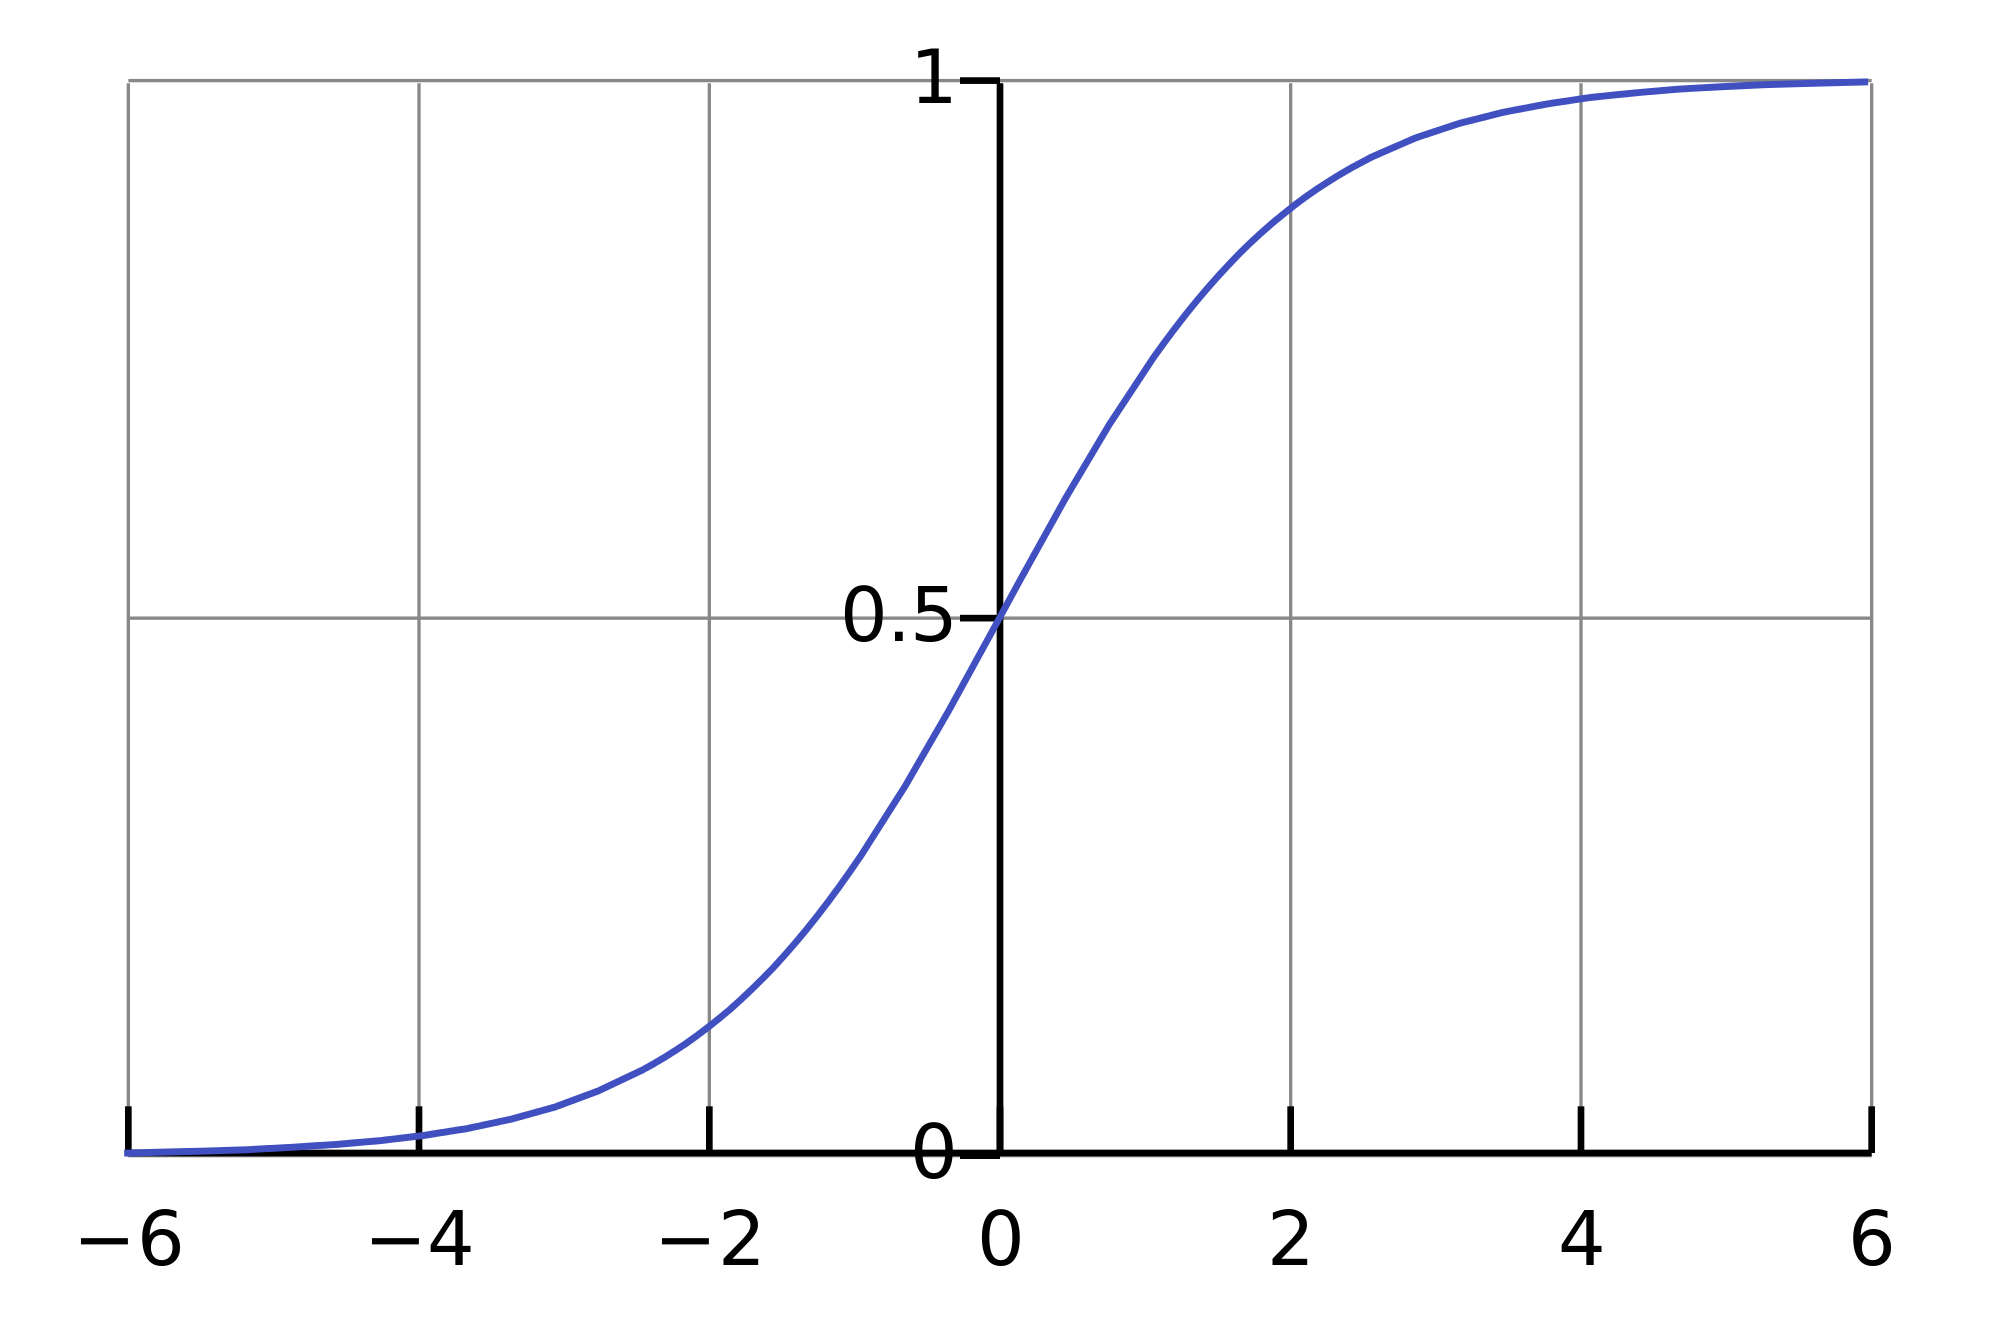
\includegraphics[width=0.95\linewidth]{../images/Logistic-curve.png}
	\caption{A graph of the logistic function.}
\end{figure}

\begin{equation}
	sigmoid(x,W,b)=1/(1+exp(Wx+b))
\end{equation}  



Often in RL the parameters of the model are denoted as θ and the goal is to optimize these parameters. For logistic regression using the sigmoid activation function this translates to θ={W,b}. Where W are the weights for the model and b is a bias for the model. Somewhat similar to the more common y=mx+b for defining a line. The b effectively shifts the sigmoid curve to the right or left.

Multidimensional Regression

This model extends to multiple dimensions or actions rather easily, $\inputVector, \basisVector$ become vectors and W is now a matrix with dimensions $len(\inputVector) x numActions$. Then the sigmoid function returns a vector of Q-values, one for each action in state \inputVector. The optimal action using the Q-Learning method can then be computed as

\[a∗= \arg\max_{a}Q(s,a)=\arg\max_{a} sigmoid(x,\theta)\]


Model Optimization 
To perform optimization of this sigmoidal model a cost function is needed. The idea of a cost function is to compute the difference between the current model and the perfect solution. For RL we use the Bellman Error to determine this
\[cost(R, S, S') = sum(0.5 * \delta(R, S, S')^{2})\]
This cost function gives a fair measure of the model error. Note, in this formulation R,S,S′ are vectors or matrices and the squared the cost is used so that positive and negative errors to not cancel each other out in the sum. It is also common to use mean in this function instead of sum because sum is effected more by variable scale. Including our model in the cost function gives

\[cost(R, S, S', \theta) = sum(0.5 * \delta(R, S, S', \theta)^{2})\]

To determine in what direction along the cost function contour will result in less error the gradient wrt the model parameters is needed 
∂cost∂W,∂cost∂b. This can be calculated in Theano rather easily.

\begin{lstlisting}
    g_W = T.grad(cost=cost, wrt=model.W)
    g_b = T.grad(cost=cost, wrt=model.b)
\end{lstlisting}

With the gradient in hand we can make a update rule to step in the direction of less cost. 
W′=W+(−∂cost∂W∗α)

b′=b+(−∂cost∂b∗α)

This can also be done in Theano rather simply as 

\begin{lstlisting}
updates = [(model.W, model.W + (-g_W * learning_rate),
           (model.b, model.b + (-g_b * learning_rate)]
\end{lstlisting}


Those are the steps needed to perform common Stochastic Gradient Descent (SGD). It should be noted that the \textit{learning rate} \learningRate for RL problems should be rather small, the effect of this will be discussed and shown later.
Model Training
Every time the agent selects an action a in some state s that leads to receiving some reward r and resulting in a new states s′ experience is gained. This single tuples of experience is kept in a experience history that is used to train the model. The experience history serves a similar purpose as training data in classification problems. 
Training the model (or updates) is done over a mini batch, where a mini batch is a randomly selected sample of from the experience history of the agent. 
Action Selection and Exploration
A common method to select an action to execute is e-greedy action selection. This algorithm simply selects one of the available actions at random with probability e. Otherwise, the selected action comes from the policy \(\pi(s)\), in this case the logistic regression model.

Learning Rate
One tough challenge that has only recently seen good solutions is deadling with highly eratic policy changes. The policy swings from one end of the spectrum to the other making it almost impossible for the optimization to eventually settle on a good policy.
Earlier I said we would look at the effect the learning rate has on the learning process. The learning rate is one of the parameters that influences the erraticness of the policy. The effect of a learning rate that is far to high is shown in the next two figures. Focus on the policy on the right that describes the optimal action/direction to be selected when the agent is in the location on the map that is the location of the arrow.


After lowering the learning rate from 0.5 to 0.01 small managable policy updates are made.

The Code 
Can be found here.

\begin{comment}
References:
1. https://en.wikipedia.org/wiki/Activation_function 
2. https://en.wikipedia.org/wiki/Q-learning 
3. http://deeplearning.net/software/theano/tutorial/examples.html#logistic-function 
4. http://deeplearning.net/tutorial/logreg.html#logreg 
5. https://webdocs.cs.ualberta.ca/~sutton/book/ebook/the-book.html 
\end{comment}